\PassOptionsToPackage{unicode=true}{hyperref} % options for packages loaded elsewhere
\PassOptionsToPackage{hyphens}{url}
%
\documentclass[ignorenonframetext,]{beamer}
\usepackage{pgfpages}
\setbeamertemplate{caption}[numbered]
\setbeamertemplate{caption label separator}{: }
\setbeamercolor{caption name}{fg=normal text.fg}
\beamertemplatenavigationsymbolsempty
% Prevent slide breaks in the middle of a paragraph:
\widowpenalties 1 10000
\raggedbottom
\setbeamertemplate{part page}{
\centering
\begin{beamercolorbox}[sep=16pt,center]{part title}
  \usebeamerfont{part title}\insertpart\par
\end{beamercolorbox}
}
\setbeamertemplate{section page}{
\centering
\begin{beamercolorbox}[sep=12pt,center]{part title}
  \usebeamerfont{section title}\insertsection\par
\end{beamercolorbox}
}
\setbeamertemplate{subsection page}{
\centering
\begin{beamercolorbox}[sep=8pt,center]{part title}
  \usebeamerfont{subsection title}\insertsubsection\par
\end{beamercolorbox}
}
\AtBeginPart{
  \frame{\partpage}
}
\AtBeginSection{
  \ifbibliography
  \else
    \frame{\sectionpage}
  \fi
}
\AtBeginSubsection{
  \frame{\subsectionpage}
}
\usepackage{lmodern}
\usepackage{amssymb,amsmath}
\usepackage{ifxetex,ifluatex}
\usepackage{fixltx2e} % provides \textsubscript
\ifnum 0\ifxetex 1\fi\ifluatex 1\fi=0 % if pdftex
  \usepackage[T1]{fontenc}
  \usepackage[utf8]{inputenc}
  \usepackage{textcomp} % provides euro and other symbols
\else % if luatex or xelatex
  \usepackage{unicode-math}
  \defaultfontfeatures{Ligatures=TeX,Scale=MatchLowercase}
\fi
% use upquote if available, for straight quotes in verbatim environments
\IfFileExists{upquote.sty}{\usepackage{upquote}}{}
% use microtype if available
\IfFileExists{microtype.sty}{%
\usepackage[]{microtype}
\UseMicrotypeSet[protrusion]{basicmath} % disable protrusion for tt fonts
}{}
\IfFileExists{parskip.sty}{%
\usepackage{parskip}
}{% else
\setlength{\parindent}{0pt}
\setlength{\parskip}{6pt plus 2pt minus 1pt}
}
\usepackage{hyperref}
\hypersetup{
            pdftitle={Introduction to R Programming},
            pdfauthor={Pedro Fonseca},
            pdfborder={0 0 0},
            breaklinks=true}
\urlstyle{same}  % don't use monospace font for urls
\newif\ifbibliography
\usepackage{color}
\usepackage{fancyvrb}
\newcommand{\VerbBar}{|}
\newcommand{\VERB}{\Verb[commandchars=\\\{\}]}
\DefineVerbatimEnvironment{Highlighting}{Verbatim}{commandchars=\\\{\}}
% Add ',fontsize=\small' for more characters per line
\usepackage{framed}
\definecolor{shadecolor}{RGB}{248,248,248}
\newenvironment{Shaded}{\begin{snugshade}}{\end{snugshade}}
\newcommand{\AlertTok}[1]{\textcolor[rgb]{0.94,0.16,0.16}{#1}}
\newcommand{\AnnotationTok}[1]{\textcolor[rgb]{0.56,0.35,0.01}{\textbf{\textit{#1}}}}
\newcommand{\AttributeTok}[1]{\textcolor[rgb]{0.77,0.63,0.00}{#1}}
\newcommand{\BaseNTok}[1]{\textcolor[rgb]{0.00,0.00,0.81}{#1}}
\newcommand{\BuiltInTok}[1]{#1}
\newcommand{\CharTok}[1]{\textcolor[rgb]{0.31,0.60,0.02}{#1}}
\newcommand{\CommentTok}[1]{\textcolor[rgb]{0.56,0.35,0.01}{\textit{#1}}}
\newcommand{\CommentVarTok}[1]{\textcolor[rgb]{0.56,0.35,0.01}{\textbf{\textit{#1}}}}
\newcommand{\ConstantTok}[1]{\textcolor[rgb]{0.00,0.00,0.00}{#1}}
\newcommand{\ControlFlowTok}[1]{\textcolor[rgb]{0.13,0.29,0.53}{\textbf{#1}}}
\newcommand{\DataTypeTok}[1]{\textcolor[rgb]{0.13,0.29,0.53}{#1}}
\newcommand{\DecValTok}[1]{\textcolor[rgb]{0.00,0.00,0.81}{#1}}
\newcommand{\DocumentationTok}[1]{\textcolor[rgb]{0.56,0.35,0.01}{\textbf{\textit{#1}}}}
\newcommand{\ErrorTok}[1]{\textcolor[rgb]{0.64,0.00,0.00}{\textbf{#1}}}
\newcommand{\ExtensionTok}[1]{#1}
\newcommand{\FloatTok}[1]{\textcolor[rgb]{0.00,0.00,0.81}{#1}}
\newcommand{\FunctionTok}[1]{\textcolor[rgb]{0.00,0.00,0.00}{#1}}
\newcommand{\ImportTok}[1]{#1}
\newcommand{\InformationTok}[1]{\textcolor[rgb]{0.56,0.35,0.01}{\textbf{\textit{#1}}}}
\newcommand{\KeywordTok}[1]{\textcolor[rgb]{0.13,0.29,0.53}{\textbf{#1}}}
\newcommand{\NormalTok}[1]{#1}
\newcommand{\OperatorTok}[1]{\textcolor[rgb]{0.81,0.36,0.00}{\textbf{#1}}}
\newcommand{\OtherTok}[1]{\textcolor[rgb]{0.56,0.35,0.01}{#1}}
\newcommand{\PreprocessorTok}[1]{\textcolor[rgb]{0.56,0.35,0.01}{\textit{#1}}}
\newcommand{\RegionMarkerTok}[1]{#1}
\newcommand{\SpecialCharTok}[1]{\textcolor[rgb]{0.00,0.00,0.00}{#1}}
\newcommand{\SpecialStringTok}[1]{\textcolor[rgb]{0.31,0.60,0.02}{#1}}
\newcommand{\StringTok}[1]{\textcolor[rgb]{0.31,0.60,0.02}{#1}}
\newcommand{\VariableTok}[1]{\textcolor[rgb]{0.00,0.00,0.00}{#1}}
\newcommand{\VerbatimStringTok}[1]{\textcolor[rgb]{0.31,0.60,0.02}{#1}}
\newcommand{\WarningTok}[1]{\textcolor[rgb]{0.56,0.35,0.01}{\textbf{\textit{#1}}}}
\usepackage{graphicx,grffile}
\makeatletter
\def\maxwidth{\ifdim\Gin@nat@width>\linewidth\linewidth\else\Gin@nat@width\fi}
\def\maxheight{\ifdim\Gin@nat@height>\textheight\textheight\else\Gin@nat@height\fi}
\makeatother
% Scale images if necessary, so that they will not overflow the page
% margins by default, and it is still possible to overwrite the defaults
% using explicit options in \includegraphics[width, height, ...]{}
\setkeys{Gin}{width=\maxwidth,height=\maxheight,keepaspectratio}
\setlength{\emergencystretch}{3em}  % prevent overfull lines
\providecommand{\tightlist}{%
  \setlength{\itemsep}{0pt}\setlength{\parskip}{0pt}}
\setcounter{secnumdepth}{0}

% set default figure placement to htbp
\makeatletter
\def\fps@figure{htbp}
\makeatother


\title{Introduction to R Programming}
\providecommand{\subtitle}[1]{}
\subtitle{Lists}
\author{Pedro Fonseca}
\date{20 Abril 2020}

\begin{document}
\frame{\titlepage}

\begin{frame}[fragile]{Preliminars}
\protect\hypertarget{preliminars}{}

The \texttt{str()} function displays the internal strucure of an object:

\begin{Shaded}
\begin{Highlighting}[]
\NormalTok{vec <-}\StringTok{ }\KeywordTok{c}\NormalTok{(}\DecValTok{1}\NormalTok{, }\DecValTok{5}\NormalTok{, }\FloatTok{0.1}\NormalTok{)}
\KeywordTok{str}\NormalTok{(vec)}
\end{Highlighting}
\end{Shaded}

\begin{verbatim}
##  num [1:3] 1 5 0.1
\end{verbatim}

\begin{Shaded}
\begin{Highlighting}[]
\NormalTok{vec_f <-}\StringTok{ }\KeywordTok{factor}\NormalTok{(}\KeywordTok{c}\NormalTok{(}\StringTok{"good"}\NormalTok{, }\StringTok{"bad"}\NormalTok{))}
\KeywordTok{str}\NormalTok{(vec_f)}
\end{Highlighting}
\end{Shaded}

\begin{verbatim}
##  Factor w/ 2 levels "bad","good": 2 1
\end{verbatim}

\begin{Shaded}
\begin{Highlighting}[]
\NormalTok{mat_char <-}\StringTok{ }\KeywordTok{matrix}\NormalTok{(}\KeywordTok{c}\NormalTok{(}\StringTok{"a"}\NormalTok{, }\StringTok{"u"}\NormalTok{, }\StringTok{"mk"}\NormalTok{, }\StringTok{"q!"}\NormalTok{), }\DataTypeTok{ncol =} \DecValTok{2}\NormalTok{)}
\KeywordTok{str}\NormalTok{(mat_char)}
\end{Highlighting}
\end{Shaded}

\begin{verbatim}
##  chr [1:2, 1:2] "a" "u" "mk" "q!"
\end{verbatim}

\end{frame}

\begin{frame}{Preliminars}
\protect\hypertarget{preliminars-1}{}

\begin{figure}
\centering
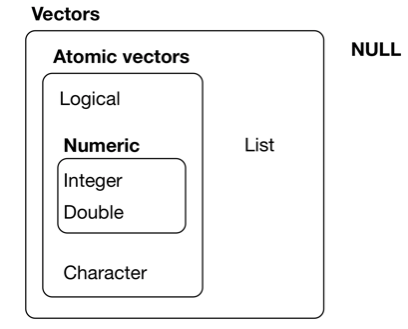
\includegraphics[width=2.60417in,height=\textheight]{figures/vec}
\caption{The hierarchy of R's vector types}
\end{figure}

\end{frame}

\begin{frame}{Why do we need lists?}
\protect\hypertarget{why-do-we-need-lists}{}

\begin{itemize}
\item
  Atomic vectors and matrices are convenient data storage structures but
  they have a limitation: all their elements have to be of the same data
  type.
\item
  If we provide elements of more than one data type to an atomic vector
  or matrix, R will coerce to the most general data type.
\end{itemize}

\end{frame}

\begin{frame}[fragile]{Why do we need lists?}
\protect\hypertarget{why-do-we-need-lists-1}{}

\begin{Shaded}
\begin{Highlighting}[]
\NormalTok{vec1 <-}\StringTok{ }\KeywordTok{c}\NormalTok{(}\OtherTok{TRUE}\NormalTok{, }\OtherTok{FALSE}\NormalTok{)}
\KeywordTok{typeof}\NormalTok{(vec1)}
\end{Highlighting}
\end{Shaded}

\begin{verbatim}
## [1] "logical"
\end{verbatim}

\begin{Shaded}
\begin{Highlighting}[]
\NormalTok{vec2 <-}\StringTok{ }\KeywordTok{c}\NormalTok{(}\OtherTok{TRUE}\NormalTok{, }\OtherTok{FALSE}\NormalTok{, }\DecValTok{3}\NormalTok{)}
\KeywordTok{typeof}\NormalTok{(vec2)}
\end{Highlighting}
\end{Shaded}

\begin{verbatim}
## [1] "double"
\end{verbatim}

Logical values are coerced to numeric if combined with numeric values.

\end{frame}

\begin{frame}[fragile]{Why do we need lists?}
\protect\hypertarget{why-do-we-need-lists-2}{}

\begin{Shaded}
\begin{Highlighting}[]
\NormalTok{vec3 <-}\StringTok{ }\KeywordTok{c}\NormalTok{(}\OtherTok{TRUE}\NormalTok{, }\OtherTok{FALSE}\NormalTok{, }\DecValTok{3}\NormalTok{, }\StringTok{"4"}\NormalTok{)}
\KeywordTok{typeof}\NormalTok{(vec3)}
\end{Highlighting}
\end{Shaded}

\begin{verbatim}
## [1] "character"
\end{verbatim}

Logical and numeric values are coerced to character if combined with
character values.

\end{frame}

\begin{frame}{What are lists?}
\protect\hypertarget{what-are-lists}{}

\begin{itemize}
\item
  Lists are a step up in complexity from atomic vectors.
\item
  Atomic vectors are homogeneous, while lists can be heterogeneous.
\item
  Lists can store objects of any type (including lists).
\item
  Lists are recursive vectors.
\end{itemize}

\end{frame}

\begin{frame}[fragile]{Creating a list}
\protect\hypertarget{creating-a-list}{}

\begin{Shaded}
\begin{Highlighting}[]
\NormalTok{my_list <-}\StringTok{ }\KeywordTok{list}\NormalTok{(}
  \KeywordTok{matrix}\NormalTok{(}\KeywordTok{c}\NormalTok{(}\DecValTok{1}\NormalTok{, }\DecValTok{5}\NormalTok{, }\DecValTok{-1}\NormalTok{, }\DecValTok{4}\NormalTok{), }\DataTypeTok{ncol =} \DecValTok{2}\NormalTok{),}
  \KeywordTok{c}\NormalTok{(}\StringTok{"S"}\NormalTok{, }\StringTok{"M"}\NormalTok{, }\StringTok{"S"}\NormalTok{, }\StringTok{"W"}\NormalTok{),}
  \StringTok{"I-am-a-string"}\NormalTok{,}
  \KeywordTok{c}\NormalTok{(}\OtherTok{TRUE}\NormalTok{, }\OtherTok{FALSE}\NormalTok{, }\OtherTok{FALSE}\NormalTok{)}
\NormalTok{)}
\end{Highlighting}
\end{Shaded}

\begin{Shaded}
\begin{Highlighting}[]
\KeywordTok{str}\NormalTok{(my_list)}
\end{Highlighting}
\end{Shaded}

\begin{verbatim}
## List of 4
##  $ : num [1:2, 1:2] 1 5 -1 4
##  $ : chr [1:4] "S" "M" "S" "W"
##  $ : chr "I-am-a-string"
##  $ : logi [1:3] TRUE FALSE FALSE
\end{verbatim}

\end{frame}

\begin{frame}[fragile]{Whats inside the list?}
\protect\hypertarget{whats-inside-the-list}{}

\begin{Shaded}
\begin{Highlighting}[]
\NormalTok{my_list}
\end{Highlighting}
\end{Shaded}

\begin{verbatim}
## [[1]]
##      [,1] [,2]
## [1,]    1   -1
## [2,]    5    4
## 
## [[2]]
## [1] "S" "M" "S" "W"
## 
## [[3]]
## [1] "I-am-a-string"
## 
## [[4]]
## [1]  TRUE FALSE FALSE
\end{verbatim}

\end{frame}

\begin{frame}[fragile]{Lists inside lists}
\protect\hypertarget{lists-inside-lists}{}

Lists can even contain other lists!

\begin{Shaded}
\begin{Highlighting}[]
\NormalTok{list_with_lists <-}\StringTok{ }\KeywordTok{list}\NormalTok{(}
  \KeywordTok{c}\NormalTok{(}\DecValTok{4}\OperatorTok{:}\DecValTok{1}\NormalTok{),}
  \KeywordTok{list}\NormalTok{(}
    \KeywordTok{matrix}\NormalTok{(}\KeywordTok{c}\NormalTok{(}\StringTok{"d"}\NormalTok{, }\StringTok{"a"}\NormalTok{, }\StringTok{"r"}\NormalTok{, }\StringTok{"r"}\NormalTok{), }\DataTypeTok{ncol =} \DecValTok{2}\NormalTok{),}
    \KeywordTok{factor}\NormalTok{(}\StringTok{"yes"}\NormalTok{, }\StringTok{"no"}\NormalTok{, }\StringTok{"yes"}\NormalTok{)}
\NormalTok{    ),}
  \KeywordTok{list}\NormalTok{(}
    \KeywordTok{c}\NormalTok{(}\OtherTok{TRUE}\NormalTok{, }\OtherTok{FALSE}\NormalTok{, }\OtherTok{TRUE}\NormalTok{),}
    \DecValTok{1}\OperatorTok{:}\DecValTok{4}\NormalTok{,}
    \KeywordTok{c}\NormalTok{(}\DecValTok{1}\NormalTok{, }\DecValTok{5}\NormalTok{, }\DecValTok{7}\NormalTok{, }\DecValTok{9}\NormalTok{, }\DecValTok{0}\NormalTok{)}
\NormalTok{    )}
\NormalTok{  )}
\end{Highlighting}
\end{Shaded}

\end{frame}

\begin{frame}[fragile]{Lists inside lists}
\protect\hypertarget{lists-inside-lists-1}{}

\begin{Shaded}
\begin{Highlighting}[]
\KeywordTok{str}\NormalTok{(list_with_lists)}
\end{Highlighting}
\end{Shaded}

\begin{verbatim}
## List of 3
##  $ : int [1:4] 4 3 2 1
##  $ :List of 2
##   ..$ : chr [1:2, 1:2] "d" "a" "r" "r"
##   ..$ : Factor w/ 1 level "yes": NA
##  $ :List of 3
##   ..$ : logi [1:3] TRUE FALSE TRUE
##   ..$ : int [1:4] 1 2 3 4
##   ..$ : num [1:5] 1 5 7 9 0
\end{verbatim}

\end{frame}

\begin{frame}[fragile]{Lists inside lists inside lists\ldots{}}
\protect\hypertarget{lists-inside-lists-inside-lists}{}

\begin{Shaded}
\begin{Highlighting}[]
\NormalTok{a_list_of_lists <-}\StringTok{ }\KeywordTok{list}\NormalTok{(}\KeywordTok{list}\NormalTok{(}\KeywordTok{list}\NormalTok{(}\KeywordTok{list}\NormalTok{(}\KeywordTok{c}\NormalTok{(}\DecValTok{1}\NormalTok{, }\DecValTok{5}\NormalTok{),}
                                       \KeywordTok{c}\NormalTok{(}\StringTok{"a"}\NormalTok{, }\StringTok{"b"}\NormalTok{)))))}
\KeywordTok{str}\NormalTok{(a_list_of_lists)}
\end{Highlighting}
\end{Shaded}

\begin{verbatim}
## List of 1
##  $ :List of 1
##   ..$ :List of 1
##   .. ..$ :List of 2
##   .. .. ..$ : num [1:2] 1 5
##   .. .. ..$ : chr [1:2] "a" "b"
\end{verbatim}

This is why lists are said to be recursive.

\end{frame}

\begin{frame}[fragile]{Naming list elements}
\protect\hypertarget{naming-list-elements}{}

\begin{Shaded}
\begin{Highlighting}[]
\KeywordTok{names}\NormalTok{(my_list) <-}\StringTok{ }\KeywordTok{c}\NormalTok{(}\StringTok{"Numbers"}\NormalTok{, }\StringTok{"Letters"}\NormalTok{,}
                    \StringTok{"a_lonely_string"}\NormalTok{, }\StringTok{"T_F"}\NormalTok{)}
\KeywordTok{str}\NormalTok{(my_list)}
\end{Highlighting}
\end{Shaded}

\begin{verbatim}
## List of 4
##  $ Numbers        : num [1:2, 1:2] 1 5 -1 4
##  $ Letters        : chr [1:4] "S" "M" "S" "W"
##  $ a_lonely_string: chr "I-am-a-string"
##  $ T_F            : logi [1:3] TRUE FALSE FALSE
\end{verbatim}

\end{frame}

\begin{frame}[fragile]{Naming list elements}
\protect\hypertarget{naming-list-elements-1}{}

\begin{Shaded}
\begin{Highlighting}[]
\NormalTok{my_list}
\end{Highlighting}
\end{Shaded}

\begin{verbatim}
## $Numbers
##      [,1] [,2]
## [1,]    1   -1
## [2,]    5    4
## 
## $Letters
## [1] "S" "M" "S" "W"
## 
## $a_lonely_string
## [1] "I-am-a-string"
## 
## $T_F
## [1]  TRUE FALSE FALSE
\end{verbatim}

\end{frame}

\begin{frame}[fragile]{Naming list elements}
\protect\hypertarget{naming-list-elements-2}{}

We can also name the elements of the list when we create it:

\begin{Shaded}
\begin{Highlighting}[]
\NormalTok{my_list <-}\StringTok{ }\KeywordTok{list}\NormalTok{(}
  \DataTypeTok{some_numbers =} \KeywordTok{matrix}\NormalTok{(}\KeywordTok{c}\NormalTok{(}\DecValTok{1}\NormalTok{, }\DecValTok{5}\NormalTok{, }\DecValTok{-1}\NormalTok{, }\DecValTok{4}\NormalTok{), }\DataTypeTok{ncol =} \DecValTok{2}\NormalTok{),}
  \DataTypeTok{some_letters =} \KeywordTok{c}\NormalTok{(}\StringTok{"S"}\NormalTok{, }\StringTok{"M"}\NormalTok{, }\StringTok{"S"}\NormalTok{, }\StringTok{"W"}\NormalTok{),}
  \DataTypeTok{a_lonely_string =} \StringTok{"I-am-a-string"}\NormalTok{,}
  \DataTypeTok{T_or_F =} \KeywordTok{c}\NormalTok{(}\OtherTok{TRUE}\NormalTok{, }\OtherTok{FALSE}\NormalTok{, }\OtherTok{FALSE}\NormalTok{)}
\NormalTok{)}

\KeywordTok{str}\NormalTok{(my_list)}
\end{Highlighting}
\end{Shaded}

\begin{verbatim}
## List of 4
##  $ some_numbers   : num [1:2, 1:2] 1 5 -1 4
##  $ some_letters   : chr [1:4] "S" "M" "S" "W"
##  $ a_lonely_string: chr "I-am-a-string"
##  $ T_or_F         : logi [1:3] TRUE FALSE FALSE
\end{verbatim}

\end{frame}

\begin{frame}[fragile]{Naming list elements}
\protect\hypertarget{naming-list-elements-3}{}

\texttt{list()} does not keep the names of input objects:

\begin{Shaded}
\begin{Highlighting}[]
\NormalTok{num_vec <-}\StringTok{ }\DecValTok{1}\OperatorTok{:}\DecValTok{3}
\NormalTok{char_mat <-}\StringTok{ }\KeywordTok{matrix}\NormalTok{(}\KeywordTok{c}\NormalTok{(}\StringTok{"a"}\NormalTok{, }\StringTok{"b"}\NormalTok{, }\StringTok{"c"}\NormalTok{, }\StringTok{"m"}\NormalTok{), }\DataTypeTok{ncol =} \DecValTok{2}\NormalTok{)}
\NormalTok{a_lonely_string <-}\StringTok{ "Hello!"}
\NormalTok{a_factor <-}\StringTok{ }\KeywordTok{factor}\NormalTok{(}\KeywordTok{c}\NormalTok{(}\StringTok{"Yes"}\NormalTok{, }\StringTok{"No"}\NormalTok{, }\StringTok{"Yes"}\NormalTok{))}

\NormalTok{my_list_}\DecValTok{2}\NormalTok{ <-}\StringTok{ }\KeywordTok{list}\NormalTok{(}
\NormalTok{  num_vec,}
\NormalTok{  char_mat,}
\NormalTok{  a_lonely_string,}
\NormalTok{  a_factor,}
\NormalTok{  my_list }
\NormalTok{  )}
\end{Highlighting}
\end{Shaded}

\end{frame}

\begin{frame}[fragile]{Naming list elements}
\protect\hypertarget{naming-list-elements-4}{}

\begin{Shaded}
\begin{Highlighting}[]
\KeywordTok{str}\NormalTok{(my_list_}\DecValTok{2}\NormalTok{)}
\end{Highlighting}
\end{Shaded}

\begin{verbatim}
## List of 5
##  $ : int [1:3] 1 2 3
##  $ : chr [1:2, 1:2] "a" "b" "c" "m"
##  $ : chr "Hello!"
##  $ : Factor w/ 2 levels "No","Yes": 2 1 2
##  $ :List of 4
##   ..$ some_numbers   : num [1:2, 1:2] 1 5 -1 4
##   ..$ some_letters   : chr [1:4] "S" "M" "S" "W"
##   ..$ a_lonely_string: chr "I-am-a-string"
##   ..$ T_or_F         : logi [1:3] TRUE FALSE FALSE
\end{verbatim}

\end{frame}

\begin{frame}[fragile]{Naming list elements}
\protect\hypertarget{naming-list-elements-5}{}

\begin{Shaded}
\begin{Highlighting}[]
\NormalTok{num_vec <-}\StringTok{ }\DecValTok{1}\OperatorTok{:}\DecValTok{3}
\NormalTok{char_mat <-}\StringTok{ }\KeywordTok{matrix}\NormalTok{(}\KeywordTok{c}\NormalTok{(}\StringTok{"a"}\NormalTok{, }\StringTok{"b"}\NormalTok{, }\StringTok{"c"}\NormalTok{, }\StringTok{"m"}\NormalTok{), }\DataTypeTok{ncol =} \DecValTok{2}\NormalTok{)}
\NormalTok{a_lonely_string <-}\StringTok{ "Hello!"}
\NormalTok{a_factor <-}\StringTok{ }\KeywordTok{factor}\NormalTok{(}\KeywordTok{c}\NormalTok{(}\StringTok{"Yes"}\NormalTok{, }\StringTok{"No"}\NormalTok{, }\StringTok{"Yes"}\NormalTok{))}

\NormalTok{my_list_}\DecValTok{2}\NormalTok{_named <-}\StringTok{ }\KeywordTok{list}\NormalTok{(}
  \DataTypeTok{numbers =}\NormalTok{ num_vec,}
  \DataTypeTok{c_mat =}\NormalTok{ char_mat,}
  \DataTypeTok{lonely =}\NormalTok{ a_lonely_string,}
  \DataTypeTok{fac =}\NormalTok{ a_factor,}
  \DataTypeTok{old_list =}\NormalTok{ my_list }
\NormalTok{  )}
\end{Highlighting}
\end{Shaded}

\end{frame}

\begin{frame}[fragile]{Naming list elements}
\protect\hypertarget{naming-list-elements-6}{}

\begin{Shaded}
\begin{Highlighting}[]
\KeywordTok{str}\NormalTok{(my_list_}\DecValTok{2}\NormalTok{_named)}
\end{Highlighting}
\end{Shaded}

\begin{verbatim}
## List of 5
##  $ numbers : int [1:3] 1 2 3
##  $ c_mat   : chr [1:2, 1:2] "a" "b" "c" "m"
##  $ lonely  : chr "Hello!"
##  $ fac     : Factor w/ 2 levels "No","Yes": 2 1 2
##  $ old_list:List of 4
##   ..$ some_numbers   : num [1:2, 1:2] 1 5 -1 4
##   ..$ some_letters   : chr [1:4] "S" "M" "S" "W"
##   ..$ a_lonely_string: chr "I-am-a-string"
##   ..$ T_or_F         : logi [1:3] TRUE FALSE FALSE
\end{verbatim}

\end{frame}

\begin{frame}[fragile]{Coercion}
\protect\hypertarget{coercion}{}

We can turn objects into a lists with \texttt{as.list()}:

\begin{Shaded}
\begin{Highlighting}[]
\NormalTok{char_vec <-}\StringTok{ }\KeywordTok{c}\NormalTok{(}\StringTok{"yes"}\NormalTok{, }\StringTok{"no"}\NormalTok{)}
\KeywordTok{as.list}\NormalTok{(char_vec)}
\end{Highlighting}
\end{Shaded}

\begin{verbatim}
## [[1]]
## [1] "yes"
## 
## [[2]]
## [1] "no"
\end{verbatim}

\begin{Shaded}
\begin{Highlighting}[]
\KeywordTok{str}\NormalTok{(}\KeywordTok{as.list}\NormalTok{(char_vec))}
\end{Highlighting}
\end{Shaded}

\begin{verbatim}
## List of 2
##  $ : chr "yes"
##  $ : chr "no"
\end{verbatim}

\end{frame}

\begin{frame}[fragile]{Coercion}
\protect\hypertarget{coercion-1}{}

\begin{Shaded}
\begin{Highlighting}[]
\NormalTok{num_matrix <-}\StringTok{ }\KeywordTok{matrix}\NormalTok{(}\DecValTok{1}\OperatorTok{:}\DecValTok{4}\NormalTok{, }\DataTypeTok{ncol =} \DecValTok{2}\NormalTok{)}
\KeywordTok{as.list}\NormalTok{(num_matrix)}
\end{Highlighting}
\end{Shaded}

\begin{verbatim}
## [[1]]
## [1] 1
## 
## [[2]]
## [1] 2
## 
## [[3]]
## [1] 3
## 
## [[4]]
## [1] 4
\end{verbatim}

\end{frame}

\begin{frame}[fragile]{Subsetting}
\protect\hypertarget{subsetting}{}

We can subset lists with:

\begin{itemize}
\tightlist
\item
  The \texttt{{[}} operator. Always returns a list.
\item
  The \texttt{{[}{[}} operator. Returns the object that is inside the
  subsetted element of the list. Can return objects of any type.
\item
  The \texttt{\$} operator. Simillar to \texttt{{[}{[}} but works only
  with named list elements.
\end{itemize}

\end{frame}

\begin{frame}[fragile]{Subsetting}
\protect\hypertarget{subsetting-1}{}

\begin{Shaded}
\begin{Highlighting}[]
\KeywordTok{str}\NormalTok{(my_list)}
\end{Highlighting}
\end{Shaded}

\begin{verbatim}
## List of 4
##  $ some_numbers   : num [1:2, 1:2] 1 5 -1 4
##  $ some_letters   : chr [1:4] "S" "M" "S" "W"
##  $ a_lonely_string: chr "I-am-a-string"
##  $ T_or_F         : logi [1:3] TRUE FALSE FALSE
\end{verbatim}

\begin{Shaded}
\begin{Highlighting}[]
\NormalTok{my_list[}\DecValTok{1}\NormalTok{] }
\end{Highlighting}
\end{Shaded}

\begin{verbatim}
## $some_numbers
##      [,1] [,2]
## [1,]    1   -1
## [2,]    5    4
\end{verbatim}

\begin{Shaded}
\begin{Highlighting}[]
\KeywordTok{typeof}\NormalTok{(my_list[}\DecValTok{1}\NormalTok{])}
\end{Highlighting}
\end{Shaded}

\begin{verbatim}
## [1] "list"
\end{verbatim}

\end{frame}

\begin{frame}[fragile]{Subsetting}
\protect\hypertarget{subsetting-2}{}

\begin{Shaded}
\begin{Highlighting}[]
\KeywordTok{is.matrix}\NormalTok{(my_list[}\DecValTok{1}\NormalTok{])}
\end{Highlighting}
\end{Shaded}

\begin{verbatim}
## [1] FALSE
\end{verbatim}

\begin{Shaded}
\begin{Highlighting}[]
\NormalTok{my_list[[}\DecValTok{1}\NormalTok{]]}
\end{Highlighting}
\end{Shaded}

\begin{verbatim}
##      [,1] [,2]
## [1,]    1   -1
## [2,]    5    4
\end{verbatim}

\begin{Shaded}
\begin{Highlighting}[]
\KeywordTok{typeof}\NormalTok{(my_list[[}\DecValTok{1}\NormalTok{]])}
\end{Highlighting}
\end{Shaded}

\begin{verbatim}
## [1] "double"
\end{verbatim}

\begin{Shaded}
\begin{Highlighting}[]
\KeywordTok{is.matrix}\NormalTok{(my_list[[}\DecValTok{1}\NormalTok{]])}
\end{Highlighting}
\end{Shaded}

\begin{verbatim}
## [1] TRUE
\end{verbatim}

\end{frame}

\begin{frame}{Subseting}
\protect\hypertarget{subseting}{}

\begin{quote}
``If list x is a train carrying objects, then x{[}{[}5{]}{]} is the
object in car 5; x{[}4:6{]} is a train of cars 4-6'' \hfill ---
@RLangTip
\end{quote}

\end{frame}

\begin{frame}[fragile]{Subsetting}
\protect\hypertarget{subsetting-3}{}

If element names are available:

\begin{Shaded}
\begin{Highlighting}[]
\NormalTok{my_list[}\StringTok{"some_letters"}\NormalTok{]}
\end{Highlighting}
\end{Shaded}

\begin{verbatim}
## $some_letters
## [1] "S" "M" "S" "W"
\end{verbatim}

\begin{Shaded}
\begin{Highlighting}[]
\NormalTok{my_list[[}\StringTok{"some_letters"}\NormalTok{]]}
\end{Highlighting}
\end{Shaded}

\begin{verbatim}
## [1] "S" "M" "S" "W"
\end{verbatim}

\begin{Shaded}
\begin{Highlighting}[]
\NormalTok{my_list}\OperatorTok{$}\NormalTok{some_letters}
\end{Highlighting}
\end{Shaded}

\begin{verbatim}
## [1] "S" "M" "S" "W"
\end{verbatim}

\end{frame}

\begin{frame}[fragile]{Subsetting}
\protect\hypertarget{subsetting-4}{}

Because it can return only a single value, you must use \texttt{{[}{[}}
with either a single positive integer or a string:

\begin{Shaded}
\begin{Highlighting}[]
\NormalTok{a_short_list <-}\StringTok{ }\KeywordTok{list}\NormalTok{(}\DataTypeTok{a =} \KeywordTok{c}\NormalTok{(}\DecValTok{1}\NormalTok{, }\DecValTok{2}\NormalTok{), }\DataTypeTok{b =} \DecValTok{3}\NormalTok{)}
\NormalTok{a_short_list[[}\DecValTok{1}\NormalTok{]]}
\end{Highlighting}
\end{Shaded}

\begin{verbatim}
## [1] 1 2
\end{verbatim}

\begin{Shaded}
\begin{Highlighting}[]
\NormalTok{a_short_list[[}\StringTok{"a"}\NormalTok{]]}
\end{Highlighting}
\end{Shaded}

\begin{verbatim}
## [1] 1 2
\end{verbatim}

\end{frame}

\begin{frame}[fragile]{Subsetting}
\protect\hypertarget{subsetting-5}{}

If you do supply a vector to \texttt{{[}{[}} it indexes recursively:

\begin{Shaded}
\begin{Highlighting}[]
\NormalTok{rec_l <-}\StringTok{ }\KeywordTok{list}\NormalTok{(}\DataTypeTok{a =} \KeywordTok{list}\NormalTok{(}\DataTypeTok{b =} \KeywordTok{list}\NormalTok{(}\DataTypeTok{c =} \KeywordTok{list}\NormalTok{(}\DataTypeTok{d =} \DecValTok{3}\NormalTok{))))}
\KeywordTok{str}\NormalTok{(rec_l)}
\end{Highlighting}
\end{Shaded}

\begin{verbatim}
## List of 1
##  $ a:List of 1
##   ..$ b:List of 1
##   .. ..$ c:List of 1
##   .. .. ..$ d: num 3
\end{verbatim}

\begin{Shaded}
\begin{Highlighting}[]
\NormalTok{rec_l[[}\StringTok{"a"}\NormalTok{]][[}\StringTok{"b"}\NormalTok{]][[}\StringTok{"c"}\NormalTok{]][[}\StringTok{"d"}\NormalTok{]] }
\end{Highlighting}
\end{Shaded}

\begin{verbatim}
## [1] 3
\end{verbatim}

\begin{Shaded}
\begin{Highlighting}[]
\NormalTok{rec_l[[}\KeywordTok{c}\NormalTok{(}\StringTok{"a"}\NormalTok{, }\StringTok{"b"}\NormalTok{, }\StringTok{"c"}\NormalTok{, }\StringTok{"d"}\NormalTok{)]] }\CommentTok{# Same as above!}
\end{Highlighting}
\end{Shaded}

\begin{verbatim}
## [1] 3
\end{verbatim}

\end{frame}

\begin{frame}[fragile]{Subsetting}
\protect\hypertarget{subsetting-6}{}

Some examples using \texttt{my\_list}:

\begin{Shaded}
\begin{Highlighting}[]
\NormalTok{my_list}
\end{Highlighting}
\end{Shaded}

\begin{verbatim}
## $some_numbers
##      [,1] [,2]
## [1,]    1   -1
## [2,]    5    4
## 
## $some_letters
## [1] "S" "M" "S" "W"
## 
## $a_lonely_string
## [1] "I-am-a-string"
## 
## $T_or_F
## [1]  TRUE FALSE FALSE
\end{verbatim}

\end{frame}

\begin{frame}[fragile]{Subsetting}
\protect\hypertarget{subsetting-7}{}

\begin{Shaded}
\begin{Highlighting}[]
\NormalTok{my_list[}\KeywordTok{c}\NormalTok{(}\DecValTok{2}\NormalTok{, }\DecValTok{3}\NormalTok{)] }
\end{Highlighting}
\end{Shaded}

\begin{verbatim}
## $some_letters
## [1] "S" "M" "S" "W"
## 
## $a_lonely_string
## [1] "I-am-a-string"
\end{verbatim}

\begin{Shaded}
\begin{Highlighting}[]
\KeywordTok{typeof}\NormalTok{(my_list[}\KeywordTok{c}\NormalTok{(}\DecValTok{2}\NormalTok{, }\DecValTok{3}\NormalTok{)]) }
\end{Highlighting}
\end{Shaded}

\begin{verbatim}
## [1] "list"
\end{verbatim}

\begin{Shaded}
\begin{Highlighting}[]
\KeywordTok{length}\NormalTok{(my_list[}\KeywordTok{c}\NormalTok{(}\DecValTok{2}\NormalTok{, }\DecValTok{3}\NormalTok{)])}
\end{Highlighting}
\end{Shaded}

\begin{verbatim}
## [1] 2
\end{verbatim}

\end{frame}

\begin{frame}[fragile]{Subsetting}
\protect\hypertarget{subsetting-8}{}

Extracting an elements from a vector that is inside a list:

\begin{Shaded}
\begin{Highlighting}[]
\NormalTok{my_list[[}\DecValTok{2}\NormalTok{]][}\DecValTok{1}\NormalTok{]}
\end{Highlighting}
\end{Shaded}

\begin{verbatim}
## [1] "S"
\end{verbatim}

or:

\begin{Shaded}
\begin{Highlighting}[]
\NormalTok{my_list[[}\KeywordTok{c}\NormalTok{(}\DecValTok{2}\NormalTok{, }\DecValTok{1}\NormalTok{)]]}
\end{Highlighting}
\end{Shaded}

\begin{verbatim}
## [1] "S"
\end{verbatim}

Extracting elements of a vector that is inside a list:

\begin{Shaded}
\begin{Highlighting}[]
\NormalTok{my_list[[}\DecValTok{2}\NormalTok{]][}\KeywordTok{c}\NormalTok{(}\DecValTok{2}\NormalTok{, }\DecValTok{3}\NormalTok{)]}
\end{Highlighting}
\end{Shaded}

\begin{verbatim}
## [1] "M" "S"
\end{verbatim}

\end{frame}

\begin{frame}[fragile]{Subsetting}
\protect\hypertarget{subsetting-9}{}

\begin{Shaded}
\begin{Highlighting}[]
\NormalTok{my_list[[}\DecValTok{1}\NormalTok{]]}
\end{Highlighting}
\end{Shaded}

\begin{verbatim}
##      [,1] [,2]
## [1,]    1   -1
## [2,]    5    4
\end{verbatim}

Extracting elements of a matrix that is inside a list:

\begin{Shaded}
\begin{Highlighting}[]
\NormalTok{my_list[[}\DecValTok{1}\NormalTok{]][, }\DecValTok{2}\NormalTok{] }\CommentTok{# Extracts the second column}
\NormalTok{my_list[[}\DecValTok{1}\NormalTok{]][}\DecValTok{1}\NormalTok{, ] }\CommentTok{# Extracts the first row}
\NormalTok{my_list[[}\DecValTok{1}\NormalTok{]][}\OperatorTok{-}\DecValTok{1}\NormalTok{, ] }\CommentTok{# Matrix without the first row}
\NormalTok{my_list[[}\DecValTok{1}\NormalTok{]][}\DecValTok{1}\NormalTok{, }\DecValTok{1}\NormalTok{] }\CommentTok{# Element in position (1,1)}
\end{Highlighting}
\end{Shaded}

\end{frame}

\begin{frame}[fragile]{Add a new element to a list using
\texttt{{[}{[}}}
\protect\hypertarget{add-a-new-element-to-a-list-using}{}

\begin{Shaded}
\begin{Highlighting}[]
\KeywordTok{length}\NormalTok{(my_list)}
\end{Highlighting}
\end{Shaded}

\begin{verbatim}
## [1] 4
\end{verbatim}

\begin{Shaded}
\begin{Highlighting}[]
\NormalTok{my_list[[}\DecValTok{5}\NormalTok{]] <-}\StringTok{ }\KeywordTok{matrix}\NormalTok{(}\KeywordTok{c}\NormalTok{(}\FloatTok{0.21}\NormalTok{, }\FloatTok{0.45}\NormalTok{, }\FloatTok{0.6}\NormalTok{, }\DecValTok{3}\NormalTok{),}
                       \DataTypeTok{ncol =} \DecValTok{2}\NormalTok{)}

\KeywordTok{length}\NormalTok{(my_list)}
\end{Highlighting}
\end{Shaded}

\begin{verbatim}
## [1] 5
\end{verbatim}

Note that this new element is not named. Using \texttt{{[}} instead of
\texttt{{[}{[}} would also work.

\end{frame}

\begin{frame}[fragile]{Add a new element to a list using \texttt{\$}}
\protect\hypertarget{add-a-new-element-to-a-list-using-1}{}

Adding elements to a list with \texttt{\$} automatically names the new
element.

\begin{Shaded}
\begin{Highlighting}[]
\NormalTok{my_list}\OperatorTok{$}\NormalTok{new_thing <-}\StringTok{ }\KeywordTok{list}\NormalTok{(}\KeywordTok{c}\NormalTok{(}\DecValTok{1}\NormalTok{, }\DecValTok{5}\NormalTok{), }\StringTok{"some-stuff"}\NormalTok{, }
                        \KeywordTok{matrix}\NormalTok{(}\DecValTok{1}\OperatorTok{:}\DecValTok{6}\NormalTok{, }\DataTypeTok{nrow =} \DecValTok{2}\NormalTok{))}
\KeywordTok{str}\NormalTok{(my_list)}
\end{Highlighting}
\end{Shaded}

\begin{verbatim}
## List of 6
##  $ some_numbers   : num [1:2, 1:2] 1 5 -1 4
##  $ some_letters   : chr [1:4] "S" "M" "S" "W"
##  $ a_lonely_string: chr "I-am-a-string"
##  $ T_or_F         : logi [1:3] TRUE FALSE FALSE
##  $                : num [1:2, 1:2] 0.21 0.45 0.6 3
##  $ new_thing      :List of 3
##   ..$ : num [1:2] 1 5
##   ..$ : chr "some-stuff"
##   ..$ : int [1:2, 1:3] 1 2 3 4 5 6
\end{verbatim}

\end{frame}

\begin{frame}[fragile]{Extracting elements from a list inside a list}
\protect\hypertarget{extracting-elements-from-a-list-inside-a-list}{}

Element 6 of \texttt{my\_list} is also list:

\begin{Shaded}
\begin{Highlighting}[]
\KeywordTok{str}\NormalTok{(my_list[}\DecValTok{6}\NormalTok{])}
\end{Highlighting}
\end{Shaded}

\begin{verbatim}
## List of 1
##  $ new_thing:List of 3
##   ..$ : num [1:2] 1 5
##   ..$ : chr "some-stuff"
##   ..$ : int [1:2, 1:3] 1 2 3 4 5 6
\end{verbatim}

\end{frame}

\begin{frame}[fragile]{Extracting elements from a list inside a list}
\protect\hypertarget{extracting-elements-from-a-list-inside-a-list-1}{}

Extract the element in the position (2, 3) of the matrix that is inside
the list that is itself inside \texttt{my\_list}:

\begin{Shaded}
\begin{Highlighting}[]
\NormalTok{my_list[[}\DecValTok{6}\NormalTok{]][[}\DecValTok{3}\NormalTok{]][}\DecValTok{2}\NormalTok{, }\DecValTok{3}\NormalTok{]}
\end{Highlighting}
\end{Shaded}

\begin{verbatim}
## [1] 6
\end{verbatim}

Since the list that inside \texttt{my\_list\_2} is named, this also
works:

\begin{Shaded}
\begin{Highlighting}[]
\NormalTok{my_list[[}\StringTok{"new_thing"}\NormalTok{]][[}\DecValTok{3}\NormalTok{]][}\DecValTok{2}\NormalTok{, }\DecValTok{3}\NormalTok{]}
\end{Highlighting}
\end{Shaded}

\begin{verbatim}
## [1] 6
\end{verbatim}

\end{frame}

\begin{frame}[fragile]{Delete a element of a list}
\protect\hypertarget{delete-a-element-of-a-list}{}

\begin{Shaded}
\begin{Highlighting}[]
\KeywordTok{str}\NormalTok{(my_list)}
\end{Highlighting}
\end{Shaded}

\begin{verbatim}
## List of 6
##  $ some_numbers   : num [1:2, 1:2] 1 5 -1 4
##  $ some_letters   : chr [1:4] "S" "M" "S" "W"
##  $ a_lonely_string: chr "I-am-a-string"
##  $ T_or_F         : logi [1:3] TRUE FALSE FALSE
##  $                : num [1:2, 1:2] 0.21 0.45 0.6 3
##  $ new_thing      :List of 3
##   ..$ : num [1:2] 1 5
##   ..$ : chr "some-stuff"
##   ..$ : int [1:2, 1:3] 1 2 3 4 5 6
\end{verbatim}

\end{frame}

\begin{frame}[fragile]{Delete an element of a list}
\protect\hypertarget{delete-an-element-of-a-list}{}

\texttt{NULL} is often used to represent the absence of a vector (as
opposed to \texttt{NA} which is used to represent the absence of a value
in a vector).

\begin{Shaded}
\begin{Highlighting}[]
\NormalTok{my_list}\OperatorTok{$}\NormalTok{new_thing <-}\StringTok{ }\OtherTok{NULL}
\CommentTok{# my_list["new_thing"] <- NULL does the same}

\KeywordTok{str}\NormalTok{(my_list)}
\end{Highlighting}
\end{Shaded}

\begin{verbatim}
## List of 5
##  $ some_numbers   : num [1:2, 1:2] 1 5 -1 4
##  $ some_letters   : chr [1:4] "S" "M" "S" "W"
##  $ a_lonely_string: chr "I-am-a-string"
##  $ T_or_F         : logi [1:3] TRUE FALSE FALSE
##  $                : num [1:2, 1:2] 0.21 0.45 0.6 3
\end{verbatim}

\end{frame}

\begin{frame}[fragile]{Delete an element of a list}
\protect\hypertarget{delete-an-element-of-a-list-1}{}

\begin{Shaded}
\begin{Highlighting}[]
\NormalTok{my_list[[}\DecValTok{5}\NormalTok{]] <-}\StringTok{ }\OtherTok{NULL}
\KeywordTok{str}\NormalTok{(my_list)}
\end{Highlighting}
\end{Shaded}

\begin{verbatim}
## List of 4
##  $ some_numbers   : num [1:2, 1:2] 1 5 -1 4
##  $ some_letters   : chr [1:4] "S" "M" "S" "W"
##  $ a_lonely_string: chr "I-am-a-string"
##  $ T_or_F         : logi [1:3] TRUE FALSE FALSE
\end{verbatim}

\end{frame}

\begin{frame}[fragile]{Delete an element of a list}
\protect\hypertarget{delete-an-element-of-a-list-2}{}

\begin{Shaded}
\begin{Highlighting}[]
\NormalTok{my_list[}\StringTok{"a_lonely_string"}\NormalTok{] <-}\StringTok{ }\OtherTok{NULL}
\CommentTok{# my_list[2] <- NULL does the same}

\KeywordTok{str}\NormalTok{(my_list)}
\end{Highlighting}
\end{Shaded}

\begin{verbatim}
## List of 3
##  $ some_numbers: num [1:2, 1:2] 1 5 -1 4
##  $ some_letters: chr [1:4] "S" "M" "S" "W"
##  $ T_or_F      : logi [1:3] TRUE FALSE FALSE
\end{verbatim}

\end{frame}

\begin{frame}[fragile]{Merge lists}
\protect\hypertarget{merge-lists}{}

You can merge lists with \texttt{c()}:

\begin{Shaded}
\begin{Highlighting}[]
\NormalTok{list1 <-}\StringTok{ }\KeywordTok{list}\NormalTok{(}\DecValTok{1}\NormalTok{, }\DecValTok{2}\NormalTok{)}
\NormalTok{list2 <-}\StringTok{ }\KeywordTok{list}\NormalTok{(}\KeywordTok{c}\NormalTok{(}\StringTok{"Sun"}\NormalTok{,}\StringTok{"Mon"}\NormalTok{), }\KeywordTok{c}\NormalTok{(}\DecValTok{1}\NormalTok{, }\DecValTok{2}\NormalTok{))}
\NormalTok{list3 <-}\StringTok{ }\KeywordTok{list}\NormalTok{(}\StringTok{"Hi!"}\NormalTok{)}

\NormalTok{merged.list <-}\StringTok{ }\KeywordTok{c}\NormalTok{(list1, list2, list3)}
\KeywordTok{str}\NormalTok{(merged.list)}
\end{Highlighting}
\end{Shaded}

\begin{verbatim}
## List of 5
##  $ : num 1
##  $ : num 2
##  $ : chr [1:2] "Sun" "Mon"
##  $ : num [1:2] 1 2
##  $ : chr "Hi!"
\end{verbatim}

\end{frame}

\begin{frame}[fragile]{Unlist}
\protect\hypertarget{unlist}{}

\begin{Shaded}
\begin{Highlighting}[]
\NormalTok{l <-}\StringTok{ }\KeywordTok{list}\NormalTok{(}
  \DataTypeTok{x =} \DecValTok{1}\OperatorTok{:}\DecValTok{2}\NormalTok{,}
  \DataTypeTok{y =} \KeywordTok{c}\NormalTok{(}\StringTok{"ab"}\NormalTok{, }\StringTok{"3"}\NormalTok{),}
  \DataTypeTok{m =} \KeywordTok{matrix}\NormalTok{(}\DecValTok{1}\OperatorTok{:}\DecValTok{4}\NormalTok{, }\DataTypeTok{ncol =} \DecValTok{2}\NormalTok{)}
\NormalTok{)}

\KeywordTok{unlist}\NormalTok{(l)}
\end{Highlighting}
\end{Shaded}

\begin{verbatim}
##   x1   x2   y1   y2   m1   m2   m3   m4 
##  "1"  "2" "ab"  "3"  "1"  "2"  "3"  "4"
\end{verbatim}

The \texttt{unlist} function:

\begin{itemize}
\tightlist
\item
  Keeps names (if available)
\item
  Collapses a list to a vector
\item
  Coerces to the most general data type
\end{itemize}

\end{frame}

\end{document}
